\documentclass{beamer}
\usepackage{tikz}
\usepackage{graphicx}
\usetikzlibrary {arrows.meta,automata,positioning}
\title{Lab 13: Statement : Create this presentation using \LaTeX, Beamer and TikZ}
\author[Author : Insert Roll No]{Author: 180010011}
\institute[IIT Dharwad]{IIT Dharwad}
\date{}
\begin{document}
\frame{\titlepage}
\frame{
\frametitle{Outline of presentation}
\begin{enumerate}
	\item Automations (restricted Turing Machines) - 2
	\pause
	\item Pictures of Turing award winners-2.
\end{enumerate}
}
\frame{
\frametitle{Automaton 1}
\begin{figure}
\centering
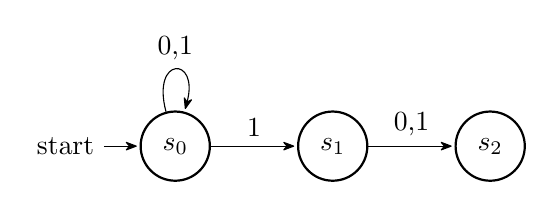
\begin{tikzpicture}[shorten >=1pt,node distance=2cm,on grid,>={Stealth[round]},every state/.style={thick}]
\node[state,initial] (s_0) {$s_0$};
\node[state] (s_1) [right = of s_0] {$s_1$};
\node[state] (s_2) [right = of s_1] {$s_2$};

\path[->] (s_0) edge[loop above] node {0,1} ()
		  (s_0) edge node [above] {1} (s_1)
		  (s_1) edge node [above] {0,1} (s_2);
\end{tikzpicture}
\caption{ X=$\{x \in \{0,1\}^*|$ the second symbol from the right is 1\}} \label{}
\end{figure}
}
\frame{
\frametitle{Automaton 2}
\begin{figure}
\centering
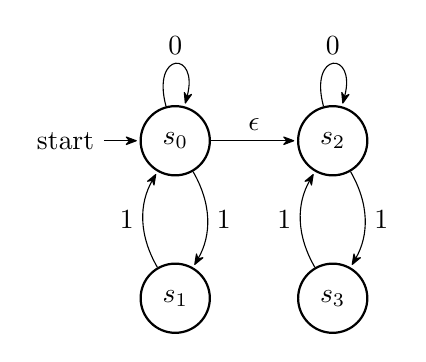
\begin{tikzpicture}[shorten >=1pt,node distance=2cm,on grid,>={Stealth[round]},every state/.style={thick}]
			\node[state,initial] (s0) {$s_0$};
			\node[state]  		 (s2) [right=of s0] {$s_2$};
			\node[state]		 (s1) [below=of s0] {$s_1$};
			\node[state]		 (s3) [below=of s2] {$s_3$};

			\path[->] (s0) edge node [above] {$\epsilon$} (s2)
					  (s0) edge[loop above] node{0} (s0)
					  (s1) edge[below,bend left] node [left] {1} (s0)
					  (s0) edge[below,bend left] node [right] {1} (s1)
					  (s2) edge[loop above] node{0} (s2)
					  (s3) edge[below,bend left] node [left] {1} (s2)
					  (s2) edge[below,bend left] node [right] {1} (s3);

\end{tikzpicture}
\caption{ X=$\{x \in \{0,1\}^*|$ the second symbol from the right is 1\}} \label{}
\end{figure}
}
\frame{
\frametitle{Turing Award Winner:1}
\begin{figure}
\centering
\begin{tikzpicture}
\node[inner sep=0pt] (Clarke) at (0,0)
    {\includegraphics[width=.29\textwidth]{edmund.jpg}};
\end{tikzpicture}
\caption{Edmund Melson Clarke received the Turing Award in the year 2007, for his work on Model Checking.} \label{}
\end{figure}
}
\frame{
\frametitle{Turing Award Winner:2}
\begin{figure}
\centering
\begin{tikzpicture}
\node[inner sep=0pt] (Lee) at (0,0)
    {\includegraphics[width=.29\textwidth]{tim.jpg}};
\end{tikzpicture}
\caption{Sir Tim Berners-Lee received the Turing Award in the year 2016,
for inventing the World Wide Web.} \label{}
\end{figure}
}
\begin{frame}
  \centering \large
  Thank you.
\end{frame}
\end{document}
